\documentclass[12pt]{article}

\usepackage[a4paper]{geometry} %page size
\usepackage{parskip} %no paragraph indentation
\usepackage{fancyhdr} %fancy stuff in page header
\pagestyle{fancy} 

\usepackage[utf8]{inputenc} %encoding
\usepackage[danish]{babel} %danish letters

\usepackage{graphicx} %import pictures
\graphicspath{ {images/} }
\usepackage{listings} %make lists

\usepackage{amsmath, amssymb, amsfonts, amsthm, mathtools} %doing math
\usepackage{algorithmicx, algpseudocode} %doing pseudocode

\title{
  Title\
  \large Subtitle
}
\author{Asger Andersen}
\date{\today}

\fancyhead{}
\lhead{Miniprojekt 2}
\rhead{Asger Andersen}

%End of preamble
%*******************************************************************************

\begin{document}

\section*{Introduktion}

Min R kode med output er vedlagt som appendix

\section{Opgave 1: Kapitalforretning}

\subsection{Delopgave a)}

Lad $x_t$ være vores kapitals størrelse i år $t$ og lad $r_t$ være renten i år. Hvis vi ingen penge bruger i år $t$, så vil vores kapital året efter (altså år $t+1$) være på 
\begin{align}
x_{t+1} = (1+r_t)x_t
\end{align}
kroner. Hvis vi udtrækker $u_t$ af kapitalen i løbet af år $t$, så vil vores kapital året efter - ifølge min logik - være på
\begin{align}
x_{t+1} = (1+r_t)(x_t - u_t)
\end{align}
kroner, da vi ikke burde få rente af den kapital, vi udtrækker. Dette svarer dog ikke helt til opgaveteksten, hvor vi tilsyneladende får rente på vores kapitals størrelse ved starten af år $t$ (før udtrækket $u_t$), da formlen her er
\begin{align}
x_{t+1} = (1+r_t)x_t - u_t
\end{align}
Jeg ved ikke meget om renter, så måske er min forståelse forkert og opgavetekstens differensligning rent faktisk en mere korrekt beskrivelse af, hvordan renter typisk fungerer.

\subsection{Delopgave b)} 

Ved konstant forretning og linært voksende udtrækning fås differensligningen
\begin{align}
x_{t+1} = (1+r)x_t - u
\end{align}
Ifølge boks 10 på side 195 i kursusbogen, er den fuldstændige løsning til denne differensligning givet ved
\begin{align}
x_t = k(1+r)^t + \frac{-u}{1 - (1+r)} = k(1+r)^t + \frac{u}{r}
\end{align}
hvor 
\begin{align}
k = x_0 - \frac{-u}{1 - (1+r)} = x_0 - \frac{u}{r}
\end{align}
Det er klart ud fra formlen for den fuldstændige løsning af differensligningen, at $x_t$ bliver negativ på et tidspunkt, hvis og kun hvis $k<0$. Dette er tilfældet, hvis og kun hvis
\begin{align}
x_0 < \frac{u}{r}
\end{align} 
Hvis vi for eksempel har, at renten er på 1 procent og vi trækker 1000 kroner ud årligt, så skal vores startkapital være på 100000 kroner eller derover, hvis vi aldrig skal gå i overtræk.

Her er et plot for værdierne af $x_t$ for $t=0,...,10$, når $r=0.015$, $u=12000$ og $x_0=200000$:
\begin{center}
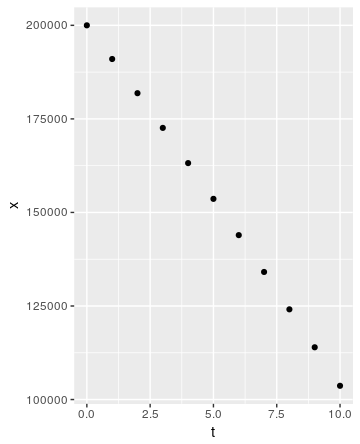
\includegraphics[scale=0.5]{q1p1.png}
\end{center}

\subsection{Delopgave c)}

Fra boks 8 side 195 i kursusbogen fås, at den fuldstændige løsning til differensligningen med konstant forretning og linært voksende udtræk er givet ved:

\begin{align}
x_t = (1+r)^{t-1}\left(x_0 + \sum_{\tau=0}^{t-1}\frac{-(u + \alpha\tau)}{(1+r)^\tau} \right)
\end{align}

Her er et plot for værdierne af $x_t$ for $t=0,...,10$, når $r=0.015$, $u=1000$, $\alpha=4000$ og $x_0=200000$:
\begin{center}
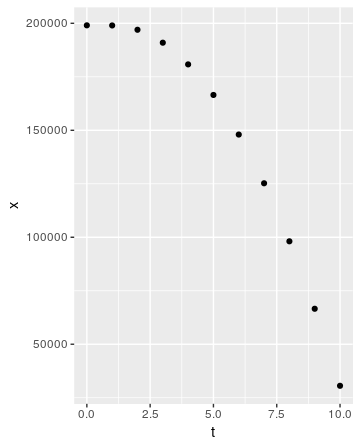
\includegraphics[scale=0.5]{q1p2.png}
\end{center}

Jeg har brugt uniroot i r til numerisk at bestemme, at hvis $r=0.015$, $u=1000$ og $x_0=200000$, så er $x_10>0$, hvis og kun hvis $\alpha<4652.81$.

\subsection{Delopgave d)}

Vi får nu differensligningen
\begin{align}
x_{t+1} = (1 + r_0r^t)x_t - (u + \alpha t)
\end{align}

Her er et plot for værdierne af $x_t$ for $t=1,...,10$, når $r_0=0.02$, $r=0.9$, $u=1000$, $\alpha=4000$ og $x_0=200000$:
\begin{center}
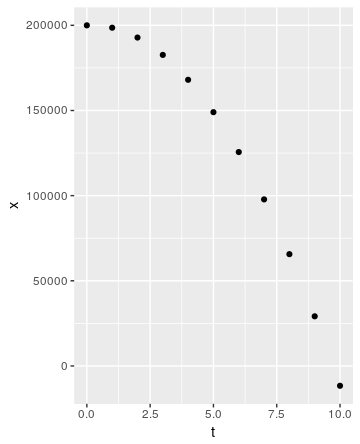
\includegraphics[scale=0.5]{q1p3.png}
\end{center}

\subsection{Delopgave e)}

Vi har nu denne differensligning
\begin{align}
x_{t+1} = \exp(r_0r^t)x_t
\end{align}
hvor $r_0=0.02$ og $r=0.9$. Ifølge boks 4 på side 194 i kursusbogen, har denne differensligning den fuldstændige løsning
\begin{align}
x_0E_t
\end{align}
hvor $x_0\in \mathbb{R}$ og 
\begin{align}
E_t = \prod_{\tau=0}^{t-1}\left( \exp(r_0r^\tau) \right) =  \exp\left(\sum_{i=0}^{t-1}r_0r^\tau\right) = \exp\left(r_0\frac{1-r^\tau}{1-r}\right)
\end{align}
Altså har differensligningen den fuldstændige løsning
\begin{align}
x_0 \exp\left(r_0\frac{1-r^\tau}{1-r}\right)
\end{align}
Den specifikke løsning for $x_0=200000$ er klar ud fra den fuldstændige løsning.

\section{Opgave b: Nationaløkonomisk model}

Lad
\begin{align}
A = \begin{bmatrix}
a  && a\\
(a-1)c && ac
\end{bmatrix}
\end{align}

Fra miniprojekt 1 ved vi, at det karakteristiske polynomien for $A$ er givet ved
\begin{align}
\rho(\lambda) = \lambda^2 + (-a(c+1))\lambda + ac
\end{align}

For $a=0.8$ og $c=3$ har dette polynomien rødderne
\begin{align}
\lambda_1=\frac{6}{5},\qquad \lambda_2 = 2
\end{align}
som altså er egenværdier for $A$. For at finde en egenvektor $q$ hørende til $\lambda_1$ skal vi løse ligningen
\begin{align}
(A-\lambda_1 E)q = 0
\end{align}
Det kan vi gøre ved rækkeoperationer
\begin{align}
\begin{bmatrix}
-\frac{2}{5} && \frac{4}{5} && 0\\
\\
\frac{-3}{5} && \frac{6}{5} && 0
\end{bmatrix}
\\
\begin{bmatrix}
-2 && 4 && 0\\
\\
-3 && 6 && 0
\end{bmatrix}
\\
\begin{bmatrix}
-2 && 4 && 0\\
\\
0 && 0 && 0
\end{bmatrix}
\\
\begin{bmatrix}
1 && -2 && 0\\
\\
0 && 0 && 0
\end{bmatrix}
\end{align}
Altså er egenvektorrummet for $\lambda_1$ givet ved
\begin{align}
\{(q_1, q_2)\in \mathbb{R}^2\ |\ q_1 = 2q_2 \}
\end{align}
Alle vektorer i dette rum er egenvektorer for $A$ hørende til egenværdien $\lambda_1$. Et eksempel på en sådan egenvektor er altså $v = (1, 2)$.

På tilsvarende vis kan vi løse ligningen
\begin{align}
(A-\lambda_2 E)q = 0
\end{align}
for at finde ud af, at egenvektorrummet for $\lambda_2$ er givet ved
\begin{align}
\{(q_1, q_2)\in \mathbb{R}^2\ |\ 3q_1 = 2q_2 \}
\end{align}
Alle vektorer i dette rum er egenvektorer for $A$ hørende til egenværdien $\lambda_2$. Et eksempel på en sådan egenvektor er altså $w = (3, 2)$.

Fra miniprojekt 1 ved jeg, at den givne nationaløkonomiske model har netop én ligevægt givet ved
\begin{align}
\begin{pmatrix}
C^*\\
I^*
\end{pmatrix}
=\begin{pmatrix}
\frac{b}{1-a}\\
0
\end{pmatrix}
\end{align}
For $a=0.8$ og $b=6$ har modellen altså denne ligevægt
\begin{align}
\begin{pmatrix}
C^*\\
I^*
\end{pmatrix}
=\begin{pmatrix}
30\\
0
\end{pmatrix}
\end{align}
Altså har den nationaløkonomiske model den fuldstændige løsning
\begin{align}
\begin{pmatrix}
C_t\\I_t
\end{pmatrix} = c_1\left(\frac{6}{5} \right)^t \begin{pmatrix} 1 \\ 2\end{pmatrix} +
c_2 2^t \begin{pmatrix} 3 \\ 2\end{pmatrix} + \begin{pmatrix}
30 \\ 0
\end{pmatrix}
\end{align}
hvor $c_1$ og $c_2$ er vilkårlige reelle tal. For at bestemme den partikulære løsning med $(C_0, I_0)=(40,9)$ skal vi løse ligningen
\begin{align}
\begin{pmatrix}
40\\9
\end{pmatrix} = c_1\left(\frac{6}{5} \right)^0 \begin{pmatrix} 1 \\ 2\end{pmatrix} +
c_2 2^0 \begin{pmatrix} 3 \\ 2\end{pmatrix} + \begin{pmatrix}
30 \\ 0
\end{pmatrix}
\end{align}
hvilket er ækvivalent med ligningen
\begin{align}
\begin{pmatrix}
10\\9
\end{pmatrix} = \begin{bmatrix}
1 && 3\\
2 && 2
\end{bmatrix} \begin{pmatrix}
c_1 \\ c_2
\end{pmatrix}
\end{align}
Vi kan for eksempel opstille totalmatricen for denne ligning og bruge rækkeoperationer til at finde ud af, at 
\begin{align}
\begin{pmatrix}
c_1\\c_2 
\end{pmatrix} = \begin{pmatrix}
\frac{7}{4}\\ \frac{11}{4}
\end{pmatrix}
\end{align}
Indsætter vi disse konstanter i den fuldstændige løsning, så får vi den søgte partikulære løsning.

\section{Opgave 3: Epidemimodel}

\subsection{Delopgave a}

Der er tale om et autonomt system af differensligninger, da tiden t kun påvirker værdien af $(S_{t+1}, I_{t+1})$ gennem værdien af $(S_t, I_t)$. Der er ikke tale om et linært system af differensligninger, da $S_{t+1}$ ikke er en linær funktion af $(S_t, I_t)$, da størrelserne $S_t^2$ og $S_tI_t$ indgår (dette kan ses ved at gange parantesen ud).

\subsection{Delopgave b, c \& d}

Lad $0 < N, b$ og $0 < a,b < 1$. 

$(S^*,I^*)\in \mathbb{R}^2$ er en ligevægt for modellen, hvis og kun hvis
\begin{align}
S^* = (1-a)S^* + bS^*\left(1 - \frac{S^* + I^*}{N} \right)\\
I^* = (1-c)I^* + aS^*
\end{align}
Det er let at se, at uanset værdien af $a, b, c$ og $N$, så vil $(S^*,I^*)=(0,0)$ altid være en løsning af disse ligninger. Ved hjælp af kedsommelige regnerier kan vi desuden komme frem til, at hvis $(S^*,I^*)\neq(0,0)$, så er $(S^*,I^*)$ en løsning til ovenstående ligningssystem, hvis og kun hvis
\begin{align}
S^* = c\Gamma(N,a,b,c), \quad I^* = a\Gamma(N,a,b,c)
\end{align}
hvor vi har defineret
\begin{align}
\Gamma(N,a,b,c) =  \frac{N(b-a)}{b(a+c)}
\end{align}
Vi ser, at modellen har en ligevægt $(S^*, I^*)$, hvor $0<S^*, I^*$, hvis og kun hvis $b>a$.

Dette passer også med, at sætter vi $N=100000, a=0.3, b=1.8$ og $c=0.1$ og fremskriver værdierne af $(S_t, I_t)$ ud fra startvektoren $(S_0, I_0)=(1000,0)$, så får vi dette plot
\begin{center}
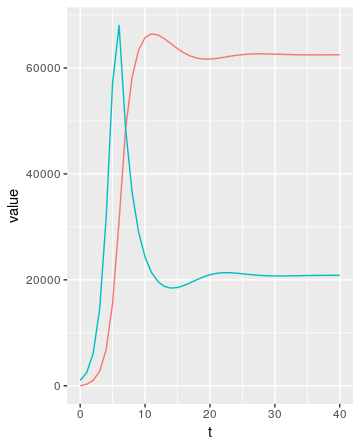
\includegraphics[scale=0.5]{q3p1.png}
\end{center}
hvor den blå graf er antallet af syge og den røde er antallet af immune. Her er $a>b$ og modellen ser ud til at have en ligevægt med $S^*$ omkring 21000 og $I^*$ omkring 62000. Laver vi samme plot med $b=0.2$, så får vi
\begin{center}
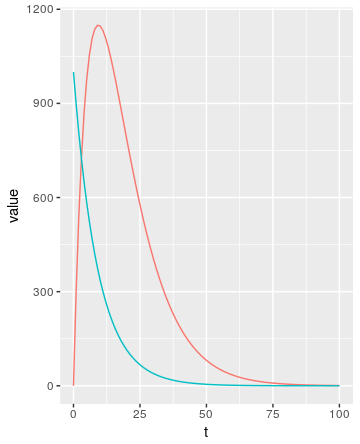
\includegraphics[scale=0.5]{q3p2.png}
\end{center}
Her er $b<a$ og modellen ser ud til at have ligevægten $(S^*, I^*)=(0,0)$. 

Lad os beregne alle ligevægte for $N=100000, a=0.3, b=1.8$ og $c=0.1$. Som sagt har vi altid ligevægten $(S^*, I^*)=(0,0)$. Bruger vi det generelle resultat fra linje (34-35), får vi desuden ligevægten $(S^*, I^*)=(20833.\overline{33},62500)$. Dette passer med, hvad vi så i plottet ovenfor.

Jeg vil nu finde ud af, om disse ligevægte er stabile. Jeg udregner funktionalmatricen for vores epidemimodel til
\begin{align}
\begin{bmatrix}
1 - a + b - b\frac{2S + I}{N} && - \frac{bS}{N} \\
\\
1-c && a 
\end{bmatrix}
\end{align}
Indsætter vi $N=100000, a=0.3, b=1.8, c=0.1, S=0$ og $I=0$ i funktionalmatricen, får vi matricen
\begin{align}
\begin{bmatrix}
2.5 && 0 \\
\\
0.9 && 0.3 
\end{bmatrix}
\end{align}
Den har egenværdierne $2.5$ og $0.3$, hvilket vil sige, at ligevægten $(0,0)$ ikke er lokalt stabilt, da $1\leq |2.5|$.

Indsætter vi $N=100000, a=0.3, b=1.8, c=0.1, S=20833.\overline{33}$ og $I=62500$ i funktionalmatricen, får vi matricen
\begin{align}
\begin{bmatrix}
0.625 && 0.375 \\
\\
0.9 && 0.3 
\end{bmatrix}
\end{align}
Den har egenværdierne $0.4625 + 0.5\overline{57}i$ og $0.4625 - 0.5\overline{57}i$, som begge har modulus $\sqrt{0.4625^2 + 0.5\overline{57}^2}=0.725<1$. Altså er ligevægten $(20833.\overline{33}, 62500)$ lokalt stabil.

\subsection{Delopgave f}

Lad $0 < N, b$ og $0 < a,b < 1$. 

$(S^*,I^*)\in \mathbb{R}^2$ er en ligevægt for den modificerede model, hvis og kun hvis
\begin{align}
S^* = (1-a)S^* + b(S^*)^2\left(1 - \frac{S^* + I^*}{N} \right)\\
I^* = (1-c)I^* + aS^*
\end{align}
Igen er det let at se, at uanset værdien af $a, b, c$ og $N$, så vil $(S^*,I^*)=(0,0)$ altid være en løsning af disse ligninger. 

For at bestemme andre løsninger til systemet, kan vi starte med at omskrive til det ækvivalente ligningssystem
\begin{align}
0 = -a + bS^*\left(1 - \frac{S^* + I^*}{N} \right)\\
I^* = \frac{a}{c}S^*
\end{align}
Indsætter vi udtrykket for $I^*$ fra den nederste ligning i den øverste, får vi
\begin{align}
0 = -a + bS^*\left(1 - \frac{S^* + \frac{a}{c}S^*}{N} \right)
\end{align}
Vi ser at dette er en andengradsligning og omskriver den til den konventionelle form
\begin{align}
0 = b\left(\frac{1 + \frac{a}{c}}{N} \right)(S^*)^2  - bS^* + a 
\end{align}
Hermed får vi diskriminanten
\begin{align}
d = (-b)^2 - 4 ab\left(\frac{1 + \frac{a}{c}}{N} \right) = b\left(b - 4a \left( \frac{1 + \frac{a}{c}}{N} \right) \right)
\end{align}
som er skarpt større end 0, hvis og kun hvis
\begin{align}
b > 4a \left( \frac{1 + \frac{a}{c}}{N} \right)
\end{align}
hvilket er ækvivalent med 
\begin{align}
\frac{4a}{b} < \frac{N}{1 + \frac{a}{c}} 
\end{align}
Antager vi dette, er diskriminanten altså skarpt større end 0. Hermed får vi altså - udover nulløsningen - to løsninger givet ved
\begin{align}
S^* = \frac{-b \pm \sqrt{d}}{2b\left(\frac{1 + \frac{a}{c}}{N} \right)}\\
I^* = \frac{a}{c}S^*
\end{align}

\end{document}